\documentclass{article}
\usepackage{enumerate}
\usepackage{amsmath}
\usepackage{amssymb}
\usepackage{graphicx}
\usepackage{subfigure}
\usepackage{geometry}
\usepackage{caption}
\usepackage{indentfirst}
\usepackage{tikz}
\usetikzlibrary{circuits.logic.US}
\usetikzlibrary{arrows.meta}
\usetikzlibrary{calc}
\geometry{left=3.0cm,right=3.0cm,top=3.0cm,bottom=4.0cm}
\renewcommand{\thesection}{Problem \arabic{section}.}
\title{VE270 Homework 3}
\author{Liu Yihao 515370910207}
\date{}

\newcommand{\drawmuxtwo}[3]{
	\draw #1 node (#2) [shape=rectangle,draw,minimum height=2cm,minimum width=2cm,text width=1cm,align=center] {#3};
	\draw (#2) ++(down:7.5mm) node {$s_0$};
	\draw (#2) ++(right:7.5mm) node {$d$};
	\draw (#2) ++(left:7.5mm) ++(up:2.5mm) node {$i_0$} ++(down:5mm) node {$i_1$};
}
\newcommand{\drawmuxfour}[3]{
	\draw #1 node (#2) [shape=rectangle,draw,minimum height=3cm,minimum width=2cm,text width=1cm,align=center] {#3};
	\draw (#2) ++(left:7.5mm) ++(up:7.5mm) node {$i_0$} ++(down:5mm) node {$i_1$} ++(down:5mm) node {$i_2$} ++(down:5mm) node {$i_3$};
	\draw (#2) ++(down:12.5mm)++(left:3.33mm) node {$s_1$} ++(right:6.66mm) node {$s_0$};
	\draw (#2) ++(right:7.5mm) node {$d$};
}
\newcommand{\drawmuxeight}[3]{
	\draw #1 node (#2) [shape=rectangle,draw,minimum height=5cm,minimum width=2cm,text width=1cm,align=center] {#3};
	\draw (#2) ++(left:7.5mm) ++(up:17.5mm) node {$i_0$} ++(down:5mm) node {$i_1$} ++(down:5mm) node {$i_2$} ++(down:5mm) node {$i_3$} ++(down:5mm) node {$i_4$} ++(down:5mm) node {$i_5$} ++(down:5mm) node {$i_6$} ++(down:5mm) node {$i_7$};
	\draw (#2) ++(down:22.5mm) node {$s_1$} ++(left:5mm) node {$s_2$} ++(right:10mm) node {$s_0$};
	\draw (#2) ++(right:7.5mm) node {$d$};
}
\newcommand{\drawdecodereight}[3]{
	\draw #1 node (#2) [shape=rectangle,draw,minimum height=5cm,minimum width=2cm,text width=1cm,align=center] {#3};
	\draw (#2) ++(right:7.5mm) ++(up:17.5mm) node {$d_0$} ++(down:5mm) node {$d_1$} ++(down:5mm) node {$d_2$} ++(down:5mm) node {$d_3$} ++(down:5mm) node {$d_4$} ++(down:5mm) node {$d_5$} ++(down:5mm) node {$d_6$} ++(down:5mm) node {$d_7$};
	\draw (#2) ++(left:7.5mm) node {$i_1$} ++(up:5mm) node {$i_0$} ++(down:10mm) node {$i_2$};
}

\begin{document}
\maketitle

\section{}
\begin{center}
	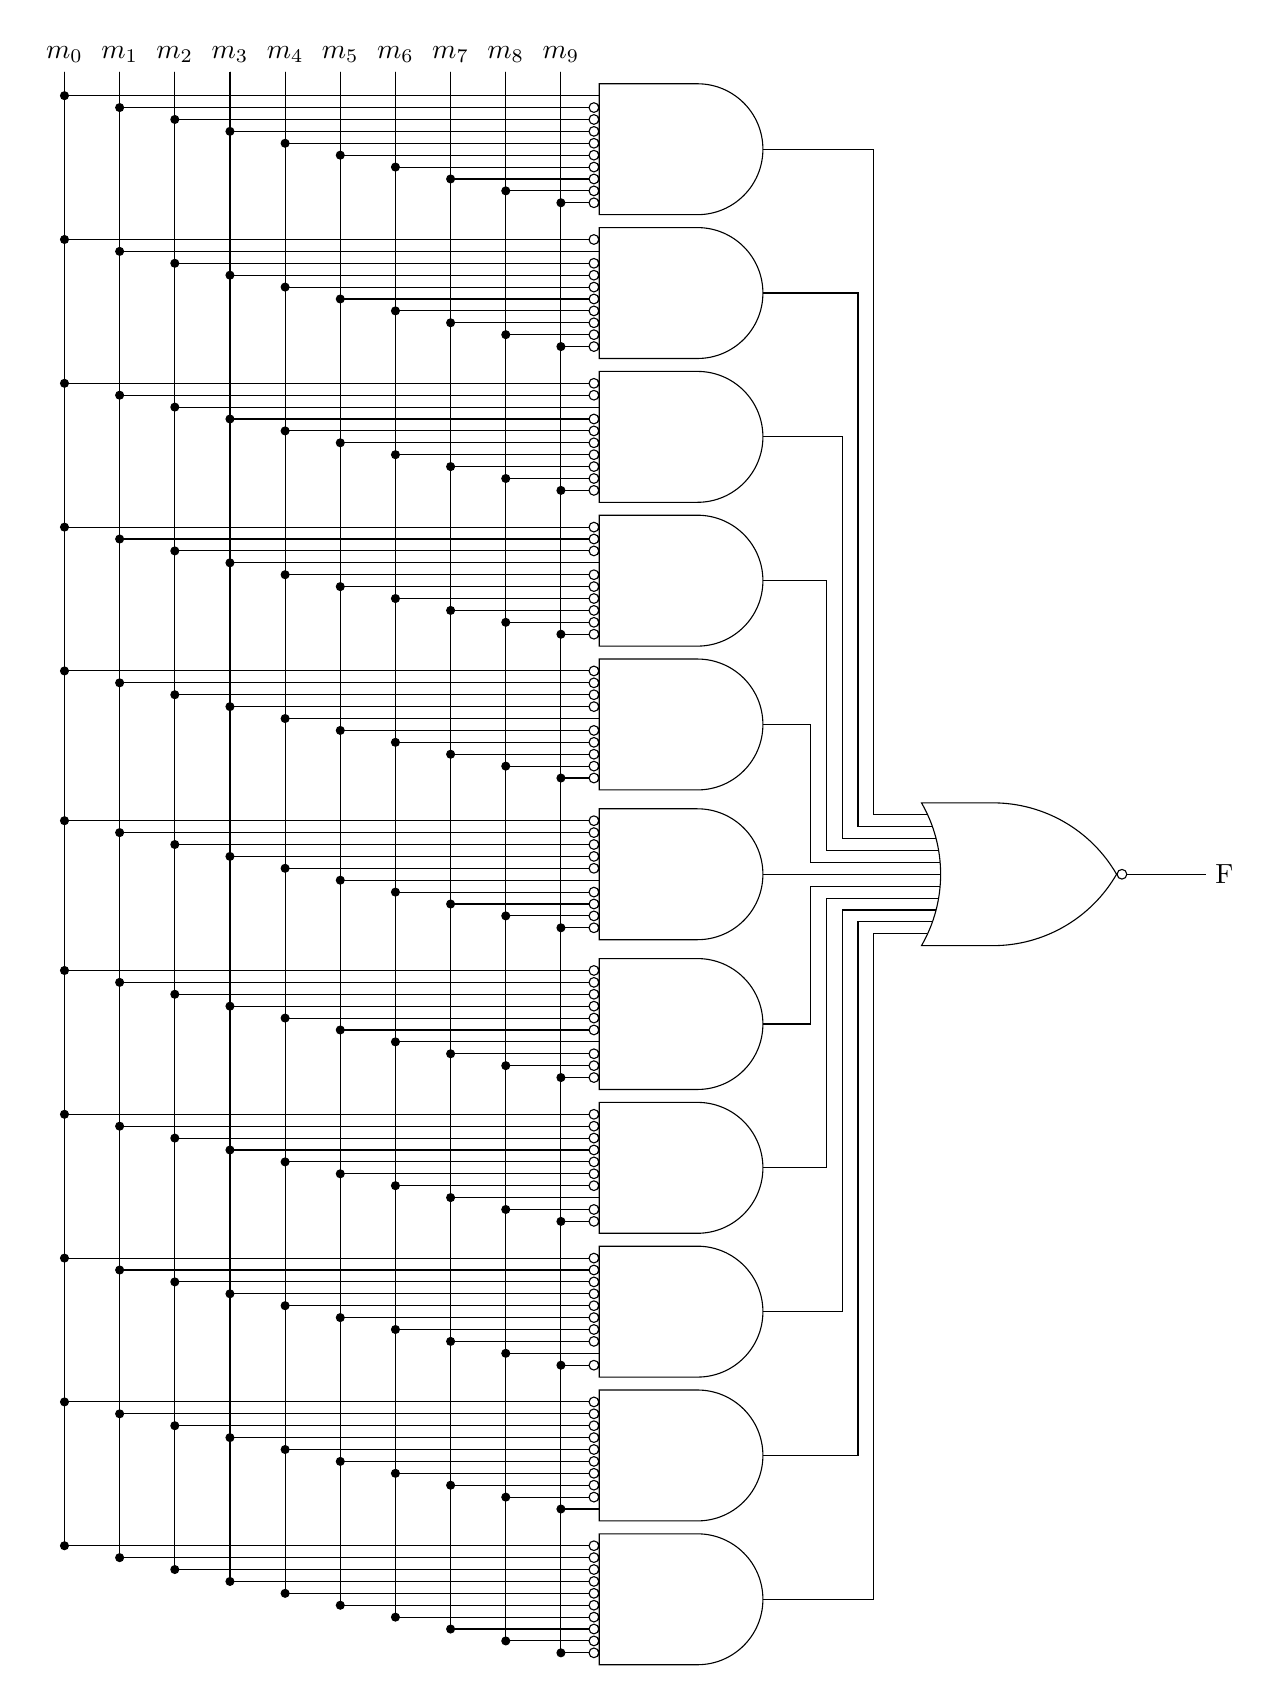
\begin{tikzpicture}[circuit logic US]
	\matrix[row sep=1.5mm]{
    		\node (m1) {$m_0$}; & \node (m2) {$m_1$}; & \node (m3) {$m_2$}; & \node (m4) {$m_3$}; & \node (m5) {$m_4$}; & \node (m6) {$m_5$}; & \node (m7) {$m_6$}; & \node (m8) {$m_7$}; & \node (m9) {$m_8$}; & \node (m10) {$m_9$}; & \\
		&&&&&&&&&& \node [and gate,inputs=niiiiiiiii] (g1) {}; \\
		&&&&&&&&&& \node [and gate,inputs=iniiiiiiii] (g2) {}; \\
		&&&&&&&&&& \node [and gate,inputs=iiniiiiiii] (g3) {}; \\
		&&&&&&&&&& \node [and gate,inputs=iiiniiiiii] (g4) {}; \\
		&&&&&&&&&& \node [and gate,inputs=iiiiniiiii] (g5) {}; \\
		&&&&&&&&&& \node [and gate,inputs=iiiiiniiii] (g6) {}; &[2cm] \node [nor gate,inputs=nnnnnnnnnnn] (g) {}; &[1cm] \node (F) {F}; \\
		&&&&&&&&&& \node [and gate,inputs=iiiiiiniii] (g7) {}; \\
		&&&&&&&&&& \node [and gate,inputs=iiiiiiinii] (g8) {}; \\
		&&&&&&&&&& \node [and gate,inputs=iiiiiiiini] (g9) {}; \\
		&&&&&&&&&& \node [and gate,inputs=iiiiiiiiin] (g10) {}; \\
		&&&&&&&&&& \node [and gate,inputs=iiiiiiiiii] (g11) {}; \\
	};
	\foreach \j / \offset in {1/14,2/12,3/10,4/8,5/6,6/6,7/6,8/8,9/10,10/12,11/14} {
		\foreach \i in {1,2,...,10} {
			\draw (m\i);
			\pgfgetlastxy{\x}{\y};
			\draw (g\j.input \i);
			\pgfgetlastxy{\xtemp}{\y};
			\filldraw (\x,\y) circle [radius=0.5mm];
			\draw (m\i) |- (g\j.input \i);
		}
		\draw (g\j.output) -- ++(right:\offset mm) |- (g.input \j);
	}
	\draw (g.output) -- (F);
	\end{tikzpicture}
\end{center}

\section{}
$$\rm C=(M_0M_1'M_2'M_3'+M_0'M_1M_2'M_3'+M_0'M_1'M_2M_3'+M_0'M_1'M_2'M_3+M_0'M_1'M_2'M_3')'$$
\begin{center}
	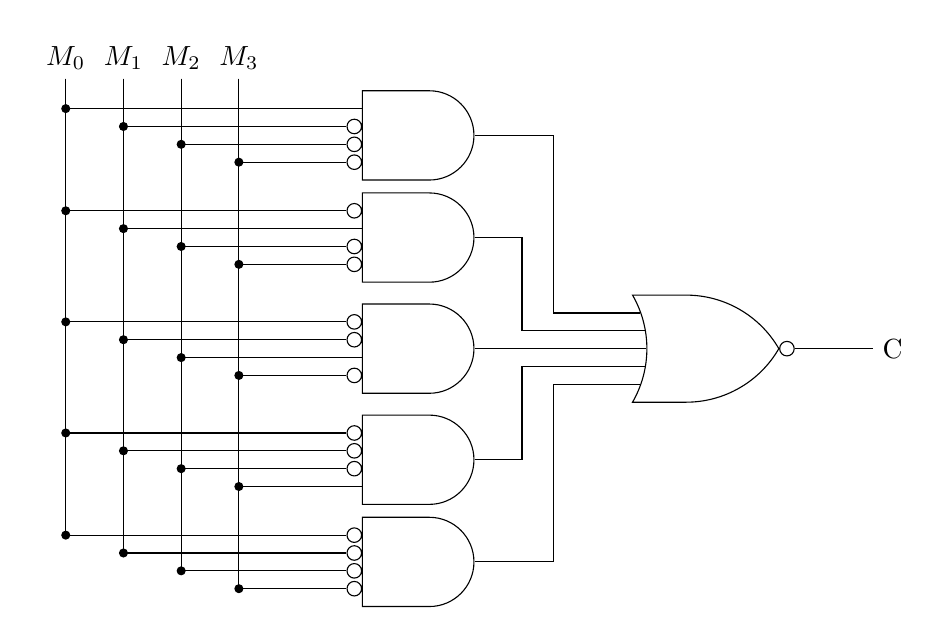
\begin{tikzpicture}[circuit logic US]
	\matrix[row sep=1.5mm]{
    		\node (m1) {$M_0$}; & \node (m2) {$M_1$}; & \node (m3) {$M_2$}; & \node (m4) {$M_3$}; &[1cm] \\
		&&&& \node [and gate,inputs=niii,scale=1.5] (g1) {}; \\
		&&&& \node [and gate,inputs=inii,scale=1.5] (g2) {}; \\
		&&&& \node [and gate,inputs=iini,scale=1.5] (g3) {}; &[2cm] \node [nor gate,inputs=nnnnn,scale=1.5] (g) {}; &[1cm] \node (C) {C}; \\
		&&&& \node [and gate,inputs=iiin,scale=1.5] (g4) {}; \\
		&&&& \node [and gate,inputs=iiii,scale=1.5] (g5) {}; \\
	};
	\foreach \j / \offset in {1/10,2/6,3/6,4/6,5/10} {
		\foreach \i in {1,2,...,4} {
			\draw (m\i);
			\pgfgetlastxy{\x}{\y};
			\draw (g\j.input \i);
			\pgfgetlastxy{\xtemp}{\y};
			\filldraw (\x,\y) circle [radius=0.5mm];
			\draw (m\i) |- (g\j.input \i);
		}
		\draw (g\j.output) -- ++(right:\offset mm) |- (g.input \j);
	}
	\draw (g.output) -- (C);
	\end{tikzpicture}
\end{center}

\section{}

Suppose $m_i$, i=0,1,2,3,4, represents the ith bit of the current tire pressure.

\begin{center}
	\begin{tikzpicture}[circuit logic US]
	\matrix[column sep=20mm]{
		\node (m0) {$m_0$}; \\
		\node (m1) {$m_1$}; \\
		\node (m2) {$m_2$}; & \node [not gate,scale=1.5] (g) {}; & \node (T) {T}; \\
		\node (m3) {$m_3$}; \\
		\node (m4) {$m_4$}; \\
	};
	\draw (m4) -- ++(right:12mm) |- (g.input) (g.output) -- (T);
	\end{tikzpicture}
\end{center}

\section{}

\begin{center}
	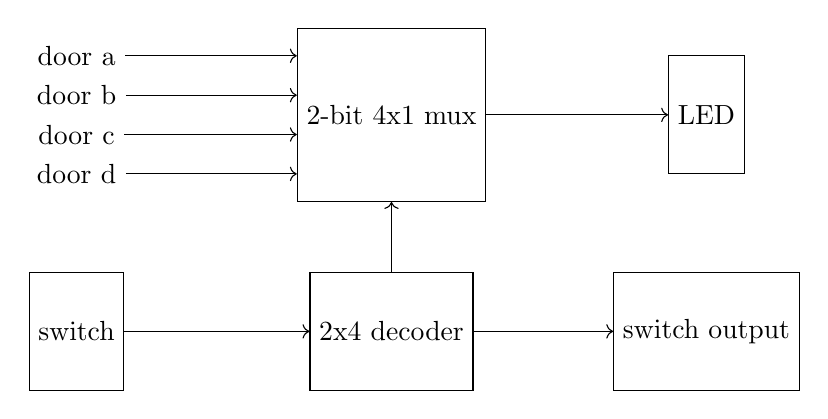
\begin{tikzpicture}
	\draw (0,0.0) node (d) {door d};
	\draw (0,0.5) node (c) {door c};
	\draw (0,1.0) node (b) {door b};
	\draw (0,1.5) node (a) {door a};
	\draw (4,0.75) node (mux) [shape=rectangle,draw,minimum height=2.2cm] {2-bit 4x1 mux};
	\draw (0,-2) node (switch) [shape=rectangle,draw,minimum height=1.5cm] {switch};
	\draw (4,-2) node (decoder) [shape=rectangle,draw,minimum height=1.5cm] {2x4 decoder};
	\draw (8,0.75) node (LED) [shape=rectangle,draw,minimum height=1.5cm] {LED};
	\draw (8,-2) node (output) [shape=rectangle,draw,minimum height=1.5cm] {switch output};
	\draw [->] (switch) -- (decoder);
	\draw [->] (decoder) -- (mux);
	\draw [->] (mux) -- (LED);
	\draw [->] (decoder) -- (output);
	\foreach \i in {a,b,c,d} {
		\draw (\i);
		\pgfgetlastxy{\xi}{\yi};
		\draw (mux.west);
		\pgfgetlastxy{\xj}{\yj};
		\draw [->] (\i) -- (\xj,\yi);
	}
	\end{tikzpicture}
\end{center}

\section{}

\begin{center}
	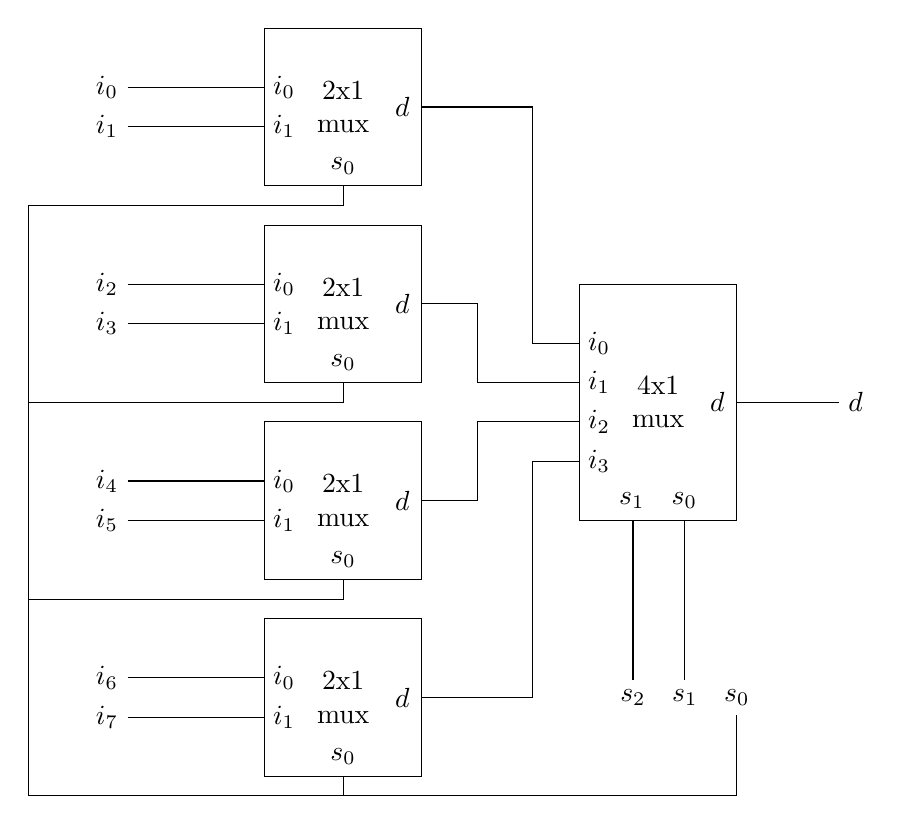
\begin{tikzpicture}
	\foreach \i in {1,2,3,4} {
		\drawmuxtwo{(0,10-2.5*\i)}{m\i}{2x1 mux};
	}
	\foreach \i/\j in {1/0,2/2,3/4,4/6} \draw (-3,10-2.5*\i+0.25) node (i\j) {$i_\j$};
	\foreach \i/\j in {1/1,2/3,3/5,4/7} \draw (-3,10-2.5*\i-0.25) node (i\j) {$i_\j$};
	\foreach \i in {0,1,...,7} {
		\draw (i\i);
		\pgfgetlastxy{\xi}{\yi};
		\draw (m1.west);
		\pgfgetlastxy{\xj}{\yj};
		\draw (i\i) -- (\xj,\yi);
	}
	\drawmuxfour{(4,3.75)}{m}{4x1 mux};
	\draw (m1.east) -- ++(right:14mm) |- ($(m.west)+(up:7.5mm)$);
	\draw (m2.east) -- ++(right:7mm) |- ($(m.west)+(up:2.5mm)$);
	\draw (m3.east) -- ++(right:7mm) |- ($(m.west)+(down:2.5mm)$);
	\draw (m4.east) -- ++(right:14mm) |- ($(m.west)+(down:7.5mm)$);
	\draw (m.east) ++(right:1.5cm) node (d) {$d$} (m) -- (d);
	\foreach \i in {0,1,2} {
		\draw (5-0.66*\i,0) node (s\i) {$s_\i$};
	}
	\draw (m.south);
	\pgfgetlastxy{\x}{\y};
	\foreach \i in {1,2} {
		\draw (s\i);
		\pgfgetlastxy{\xx}{\yy};
		\draw (s\i) -- (\xx,\y);
	}
	\draw (s0) -- (5,-1.25) -| (m4) (5,-1.25) -- (-4,-1.25) -- (-4,6.25);
	\foreach \i in {1,2,3} \draw (-4,8.75-2.5*\i) -| (m\i.south);
	\end{tikzpicture}
\end{center}

\section{}
\begin{center}
	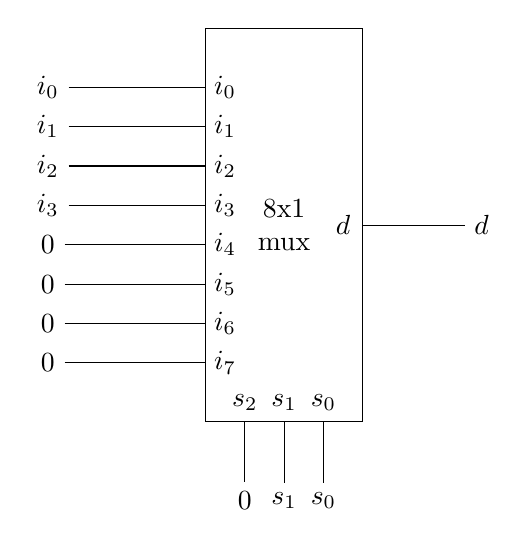
\begin{tikzpicture}
	\drawmuxeight{(0,0)}{m}{8x1 mux};
	\draw (m.east) ++(right:1.5cm) node (d) {$d$} (m) -- (d);
 	\foreach \i in {0,...,3} {
 		\draw (-3,1.75-0.5*\i) node (i\i) {$i_\i$};
 		\draw (i\i) -- (-1,1.75-0.5*\i);
 	}
 	\foreach \i in {4,...,7} {
 		\draw (-3,1.75-0.5*\i) node (i\i) {0};
 		\draw (i\i) -- (-1,1.75-0.5*\i);
 	}
 	\draw (-0.5,-3.5) node (s2) {0} (0,-3.5) node (s1) {$s_1$} (0.5,-3.5) node (s0) {$s_0$};
 	\draw (s2) -- (-0.5,-2.5) (s1) -- (0,-2.5) (s0) -- (0.5,-2.5);
	\end{tikzpicture}
\end{center}

\section{}
$$\rm F=c'+ab'$$
\begin{center}
	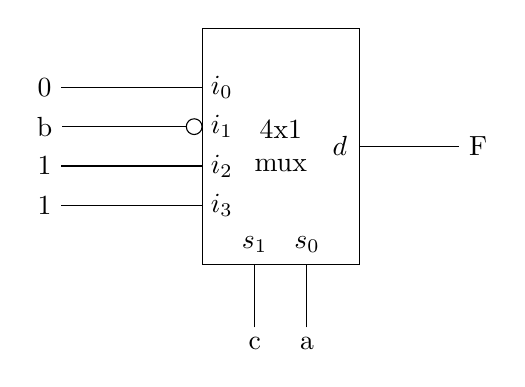
\begin{tikzpicture}
	\drawmuxfour{(0,0)}{m}{4x1 mux};
	\draw (m.east) ++(right:1.5cm) node (F) {F} (m) -- (F);
 	\draw (-3,0.75) node (i0) {0} (i0) -- (-1,0.75);
 	\draw (-3,0.25) node (i1) {b} (i1) -- (-1.2,0.25);
 	\draw (-1.1,0.25) circle[radius=1mm];
 	\draw (-3,-0.25) node (i2) {1} (i2) -- (-1,-0.25);
 	\draw (-3,-0.75) node (i3) {1} (i3) -- (-1,-0.75);
 	\draw (-0.33,-2.5) node (c) {c} (0.33,-2.5) node (a) {a};
 	\draw (c) -- (-0.33,-1.5) (a) -- (0.33,-1.5);
	\end{tikzpicture}
\end{center}

\section{}
$$\rm F=c'+ab'$$
\begin{center}
	\begin{tikzpicture}[circuit logic US]
	\drawdecodereight{(0,0)}{m}{3x8 decoder};
	\draw (4,0.25) node [nor gate,inputs=nnn,scale=2] (g) {};
	\draw (1,1.25) -- ++(right:1cm) |- (g.input 1);
	\draw (1,0.25) -- (g.input 2);
	\draw (1,-1.75) -- ++(right:1cm) |- (g.input 3);
	\draw (g.output) ++(right:1.5cm) node (F) {F} (g.output) -- (F);
	\foreach \i / \j in {1/c,2/b,3/a} {
		\draw (-3,1-0.5*\i) node (\j) {\j};
		\draw (\j) -- (-1,1-0.5*\i);
	}
	\end{tikzpicture}
\end{center}



\end{document}
